\documentclass{article}
\usepackage{amsmath,amstext,amssymb}
\usepackage[ttscale=0.7]{libertine}
\usepackage[libertine]{newtxmath}
\usepackage{siunitx}
\usepackage{inconsolata}
\usepackage{wrapfig}

\usepackage{sectsty}
\allsectionsfont{\sffamily}

\usepackage{xcolor}
\usepackage[colorlinks=true,
            linkcolor=blue,
            urlcolor=blue,
            breaklinks,
            pdftex,
            allbordercolors=white]{hyperref}
\usepackage{graphicx}
\usepackage{booktabs}
\usepackage{chemformula}
\usepackage{parskip}

\usepackage{listings}

\usepackage{datetime2}
\renewcommand{\DTMdisplaydate}[4]{#1-#2-#3}

\begin{document}

\lstset{language=XML,stringstyle=\ttfamily}

\begin{center}
	\Large{\textbf{\sffamily{Setting Up THAMES v5.0 Input}}}
\end{center}
\begin{center}
	\large{Jeffrey W. Bullard}
\end{center}
\begin{center}
	\large{\DTMnow}
\end{center}

\vspace{0.25truein}
\tableofcontents

\vspace{0.25truein}
This document provides guidance on how to prepare input files for THAMES v5.0. Special
attention is given to common pitfalls to avoid and some troubleshooting recommendations
for fixing improper input files.

\section{\label{sec:requirements} Software Requirements}
The following software must be installed and running properly on your computer:
\begin{itemize}
	\item GEMS3K standalone library 3.4.1: \href{http://gems.web.psi.ch/GEMS3K/downloads/index.html}{http://gems.web.psi.ch/GEMS3K/downloads/index.html}
	\item THAMES v5.0: \href{https://github.tamu.edu/jwbullard/THAMES.git}{https://github.tamu.edu/jwbullard/THAMES.git}
	\item (Optional) GEM-Selektor 3.6.0 or 3.7.0: \href{http://gems.web.psi.ch/GEMS3/downloads/index.html}{http://gems.web.psi.ch/GEMS3/downloads/index.html}
\end{itemize}

\section{\label{sec:categories} Categories of THAMES Input}
Throughout this document, it will be assumed that your THAMES simulation will happen
in a working directory called \verb!$WORKDIR!.

THAMES requires three categories of input files:
\begin{enumerate}
	\item The initial 3D microstructure of the material system
	\item Thermodynamic data input files produced by GEM-Selektor
	\item Microstructure input file and file linking microstructure phases to GEM phases
	\item Files to specify calculation times and microstructure output times
	\item (Optional) File containing standard input to redirect to the program
\end{enumerate}
Each of these will be detailed in the following sections.

\subsection{Microstructure initial 3D arrangement}
The microstructure representation is a digitized 3D image with \verb!X_Size! voxels
in the $x$ direction, \verb!Y_Size! in the $y$ direction, and \verb!Z_Size!
in the $z$ direction.  Each voxel is a physical dimension of
\verb!Image_Resolution! in micrometer units.
This is a normal ASCII text file.  The first few lines of an example microstructure
are given below.

\scriptsize{
	\begin{lstlisting}
#THAMES:Version: 5.0
#THAMES:X_Size: 100
#THAMES:Y_Size: 100
#THAMES:Z_Size: 100
#THAMES:Image_Resolution: 1.0
1
1
1
2
1
2
1
.
.
.
\end{lstlisting}
}

\normalsize{ }
The meaning of the five lines of header information follows:
\begin{itemize}
	\item \verb!#THAMES:Version! is the THAMES version with which these data
	      should be compatible. It is not currently used in the code but is only for
	      informational purposes;
	\item \verb!#THAMES:X_Size!, \verb!#THAMES:Y_Size!, and \verb!#THAMES:Z_Size!
	      are the system dimensions, in voxel units, in all three Cartesian
	      directions;
	\item \verb!#THAMES:Image_Resolution! is the linear dimension of each cubic
	      voxel, in \unit{\micro\meter} units.
\end{itemize}

After the five-line header to this file, each line contains a single integer corresponding to the ID of
one of the microstructure phases (not the GEM phases).  The rows have a
\verb!z-y-x! nesting convention, by the first voxel is $(0,0,0)$, the $x$ coordinates
vary most quickly and the $z$ coordinates vary most slowly.

One way to generate such a file is to create a virtual 3D microstructure using VCCTL,
which produces a \verb!.img! file in much the same format as just shown.  However,
the VCCTL phase ID numbers (Table~\ref{tab:vcctlphases}) are different than the
ones required by THAMES.  Therefore, one must replace
the VCCTL ID numbers with the corresponding THAMES microstructure id numbers.
A C program called \verb!vcctl2thames! has been provided to assist with this, but the
program may need to be edited as needed to be consistent with the THAMES microstructure
definition file described later in this document.

\small{
	\begin{table}
		\caption{\label{tab:vcctlphases} VCCTL 9.5 phase identification numbers}
		\begin{tabular}{lSlSlS} \toprule
			Phase       & \multicolumn{1}{c}{ID} &
			Phase       & \multicolumn{1}{c}{ID} &
			Phase       & \multicolumn{1}{c}{ID}                                                             \\ \midrule
			Water       & 0                      & Gypsum                  & 7  & \ch{Ca(OH)2}          & 19 \\
			Void        & 55                     & Bassanite (Hemihydrate) & 8  & \ch{C-S-H}            & 20 \\
			Alite       & 1                      & Anhydrite (\ch{CaSO4})  & 9  & \ch{C3AH6}            & 21 \\
			Belite      & 2                      & Silica Fume             & 10 & Ettringite            & 22 \\
			\ch{C3A}    & 3                      & Inert                   & 11 & \ch{Fe(OH)3}          & 25 \\
			\ch{C4AF}   & 4                      & Silica glass            & 16 & Pozzolanic \ch{C-S-H} & 26 \\
			\ch{K2SO4}  & 5                      & Monosulfate             & 24 & Friedel salt          & 29 \\
			\ch{Na2SO4} & 6                      & Monocarboaluminate      & 34 & \ch{CaCl2}            & 28 \\
			\ch{CaCO3}  & 33                     & Str{\"{a}}tlingite      & 30 & Brucite               & 35 \\ \bottomrule
		\end{tabular}
	\end{table}
}

\subsection{\label{sec:thermodata} Thermodynamic data input}
THAMES 5.0 comes with the thermodynamic data files you will need to run most
of the simulations you want. This includes systems with temperatures ranging
from \qty{283}{\kelvin} to \qty{333}{\kelvin} and including most of the
important components of portland cement, portland limestone cement, and oil well
cement. It also includes most of the iron sulfides needed for simulations
involving pyrrhotite oxidation, as well as some common supplementary
cementitious materials (SCMs) including silica fume and proxies for the main
glassy and crystalline phases found in fly ashes. A full list of all the phases
included can be found in the appendix.

The thermodynamic data files can be found in any of the various test cases
provided with THAMES 5.0, located in subfolders of the \verb!tests! folder:
\begin{itemize}
	\item \verb!alite-298K-sealed-wc35!
	\item \verb!highvolume-silicafume!
	\item \verb!PC-Carbonate-200!
	\item \verb!PC-FlyAsh-200!
	\item \verb!portcem-298K-sat-wc45!
	\item \verb!portcem-298K-sealed-alk-wc45!
	\item \verb!portcem-298K-sealed-wc45!
	\item \verb!pyrragg-298K-sat!
	\item \verb!pyrrcem-296K-sat!
\end{itemize}
The first seven test cases in this list all have the exact same thermodynamic
data files, a collection of five files that all start with \verb!thames-!
The last two test cases have data files that contain chlorinated phases such
as Friedel's salt and Kuzel's salt, but they do not contain the glassy and
crystalline fly ash components.

If you need a system that cannot be modeled with these thermodynamic
data files, you will need to use the GEM-Selektor software specified in
Section~\ref{sec:requirements} and follow its documentation for creating
recipes and exporting data files.

\normalsize{ }
\subsubsection{\label{sec:thermodataformat} Meaning of GEMS3K the File Contents}
For normal usage of THAMES, one does not need to be concerned with most of the contents of
the GEMS3K files.  However, a few noteworthy items are as follows:
\begin{itemize}
	\item The \verb!-dat.lst! file contains that string that the GEMS3K library reads when
	      performing a calculation so that it knows which other files contain the thermodynamic
	      data it needs to run.
	\item The \verb!-dch.dat! file contains the names of the independent components
	      in the \verb!<ICNL>! field, the names of the dependent components in the
	      \verb!<DCNL>! field, and the names of the phases in the \verb!<PHNL>! field.
	      You will need these names when correlating microstructure phases with GEM phases.
	      This file also contains the parameters needed to calculate the molar volumes
	      and densities of the dependent components as a function of temperature and pressure.
	\item The \verb!-dbr.dat! file contains information about the calculated state of
	      the system calculated using GEM Selektor, such as the activity coefficients,
	      and phase abundances.  But these will change with subsequent calculations in
	      THAMES and so they are not of concern in the great majority of cases.
	\item The \verb!-ipm.dat! file contains information about the numerical parameters
	      used in the calculations, and are not of immediate concern for using THAMES.
\end{itemize}

%\fbox{
%\begin{minipage}{0.9\textwidth}
%    \textbf{WARNING}:  With the sole exception of the modification to the
%    \texttt{-sol-dat.lst} file already described, you must \textsc{not} modify
%    any of the other GEMS3K input files.  Doing so will likely cause the simulation
%    to crash with a GEM error.
%\end{minipage}
%}

\subsection{\label{sec:materialsystemfiles} Simulation Parameters}
\subsubsection{\label{sec:microphasedefs} Microstructure phase definition
	section}
THAMES defines a collection of phases that can potentially be present in its
3D microstructure. These are called ``(THAMES) microstructure phases,'' and
they can be defined as one or more of the phases recognized in the
thermodynamic data files from GEMS. For example, one microstructure phase
could be defined for each of the multiple phases in AFm family that
GEMS recognizes, or one microstructure phase could be defined as
the collection of all of those AFm phases. The user has the liberty to
define these microstructure phases, and it is not necessary to include
every phase recognized by GEMS within the collection of microstructure phases.
If you know that silica fume will never be present within your simulation,
it does not need to be defined in any microstructure phase that you create.
However, two non-negotiable microstructure phases \textbf{must} always be defined:
\textit{void space} and \textit{electrolyte} (the aqueous pore solution).

The other information that must be given is the final age of the system
to be simulated and the specific times that you want to output
microstructure images. These are both given in units of days.

The file for specifying these simulation parameters
in a JSON file, which you can name anything you want but which has a default
name of \verb!simparams.json!. The documentation for JSON syntax can be found at
\href{https://www.json.org}{https://www.json.org}.
We will examine the typical contents of this file for a portland
cement paste with some pyrrhotite included.

\subsubsection{\label{sec:envsection} Environment section.}
The first section is called \verb!environment! and contains
information about the curing conditions and any boundary conditions
on the electrolyte composition. An example is shown below, with
extra annotations that are not included in the actual JSON file

\scriptsize{
	\begin{lstlisting}
{
  "environment": {
    "temperature": 296.15,        # Curing temperature (K), required
    "reftemperature": 298.15,     # Reference temperature (K) for kinetics, required
    "saturated": 1,               # 1 = saturated pores, 0 = sealed pores,
    "electrolyte_conditions": [   # (optional)
      { "DCname": "Ca(CO3)@", "condition": "initial", "concentration": 1.0e-6 },
      { "DCname": "AlO2H@", "condition": "initial", "concentration": 1.0e-6 },
      { "DCname": "CaSiO3@", "condition": "initial", "concentration": 1.0e-6 },
      { "DCname": "Fe(CO3)@", "condition": "initial", "concentration": 1.0e-6 },
      { "DCname": "MgSiO3@", "condition": "initial", "concentration": 1.0e-6 },
      { "DCname": "KOH@", "condition": "initial", "concentration": 1.0e-6 },
      { "DCname": "Ca(SO4)@", "condition": "initial", "concentration": 1.0e-6 },
      { "DCname": "K+", "condition": "initial", "concentration": 2.0e-6 },
      { "DCname": "SO4-2", "condition": "initial", "concentration": 1.0e-6 },
      { "DCname": "Na+", "condition": "initial", "concentration": 0.672 },
      { "DCname": "ClO-", "condition": "initial", "concentration": 0.672 }
    ],
  },
  .
  .
  .
}
\end{lstlisting}
}

\normalsize{ }
The \verb!temperature!, \verb!reftemperature!, and \verb!saturated! lines
are required for every simulation. The \verb!electrolyte_conditions! section
is techincally optional, but it is a good idea to have it. The GEMS library
used by THAMES is more likely to properly converge if there is at least a little
bit of each independent component in the electrolyte at the beginning. As shown,
this can be done by including small amounts of different dependent components
(DCs) that contain the ICs.

The list of all available DCs can be found in the \verb!DCNL! section of the
thermodynamic DCH file (usually called \verb!thames-dch.dat!).
The required options for any electrolyte component are:
\begin{itemize}
	\item \verb!DCname!, must exacdtly match a name in the \verb!DCNL! section
	      of the \verb!-dch.dat! file.
	\item \verb!condition! can be ``initial'' if the component's concentration
	      is to be set initially but can vary as the simulation proceeds, or ``fixed''
	      if the component's concentration is to remain at the same value throughout.
	\item \verb!concentration! is the molal concentration for the component in
	      units of moles per kilogram of water.
\end{itemize}
Please be aware that the net electrical charge of the electrolyte must
be zero, and it is the user's reponsibility to ensure that the concentrations
are set in a way to balance the charge. If the charge is \textbf{not} balanced,
the simulation will throw an exception and exit.

\subsubsection{\label{sec:microphases} Microstructure phase definitions}
The next section is called \verb!microstructure! and defines each
of the phases (or collection of phases) that can potentially exist
within the 3D microstructure. The characteristics of a microstructure
phase definition are
\begin{itemize}
	\item its name,
	\item a unique numerical identification number (id) (\textbf{Note}
	      that each id appearing in the initial 3D microstructure image
	      file must be equal to the numerical id for one of the microstructure
	      phases defined here),
	\item whether or not it is considered to be part of the cementitious
	      material or is some other component in the mixture,
	\item its relation to phases defined in the thermodynamic data,
	\item its internal, or ``subvoxel'' porosity (assumed to be zero if
	      not given),
	\item its internal pore size distribution (optional),
	\item information about its kinetic behavior (more details to follow below),
	      and
	\item the color it should have in visualizations produced by THAMES
\end{itemize}

The section opens with its name (microstructure) and the number
of microstructure phases that are defined
\scriptsize{
\begin{lstlisting}
  "microstructure": {
    "numentries": 23,
    .
    .
    .
  },
\end{lstlisting}

\normalsize{ }
In this example there are going to be 23 microstructure phases
defined. Remember that every phase in the microstructure must be
defined here, but that not every phase defined here must appear
in the microstructure.
Immediately after the \verb!numentries!, each phase is
defined sequentially in a collection named \verb!phases!.

\paragraph{The void phase.} The first defined phase \textit{must} be ``Void'' which
is just empty porosity within the microstructure. This phase is unique
because it is the only one that does not have any associated thermodynamic
phase. The meaning of each entry is
\scriptsize{
	\begin{lstlisting}
    "phases": [
      {
        "thamesname": "Void",
        "id": 0,
        "cement_component": 0,
        "display_data": { "red": 0.0, "green": 0.0, "blue": 0.0, "gray": 0.0 }
       },
       .
       .
       .
    ],
  },
\end{lstlisting}
}

\normalsize{ }
The meaning of each entry is
\begin{itemize}
	\item \verb!thamesname! is any string in quotes to designate the phase.
	      The void phase \textbf{must} be named \verb!Void! and the pore
	      solution phase \textbf{must} be named \verb!Electrolyte!, but
	      you are free to choose the names of all other microstructure phases.
	\item  \verb!id! is the unique numerical identification number, which
	      must be a non-negative integer. The void phase \textbf{must} have
	      \verb!id! of 0 and the pore solution \textbf{must} have
	      \verb!id! of 1, but you are free to choose the \verb!id!
	      of all other microstructure phases. Just remember that the phase
	      identificatino numbers in the 3D microstructure image file must
	      correspond to the correct microstructure phase \verb!id! here.
	\item \verb!cement_component! is 1 for any phase that is solid and
	      that belongs to the cementitious material, such as cement clinker phases, gypsum,
	      alkali sulfates, free lime, \textit{etc}, and is 0 for other
	      phases such as void, electrolyte, silica fume, fly ash phases, and
	      any solid hydration products such as \ch{C-S-H} gel. This distinction
	      is needed for internal calculations of water/cement ratio and
	      water/solids ratio.
	\item \verb!display_data! is a set of red/green/blue/gray values
	      that specify the color of the phase in THAMES visualizations. Many
	      microstructure phases, though not all, have default colors assigned
	      already according to predefined \verb!thamesname! names, so this entry
	      is only needed if you are defining a new
	      microstructure phase, changing the name of an existing phase,
	      or if you wish to override the default color.
\end{itemize}

\paragraph{The electrolyte phase.} The next phase after the void phase
\textbf{must} be the pore solution, which has the name \verb!Electrolyte!:
\scriptsize{
	\begin{lstlisting}
  {
    "thamesname": "Electrolyte",
    "id": 1,
    "cement_component": 0,
    "gemphase_data": [
      {
        "gemphasename": "aq_gen",
        "gemdc": [
          { "gemdcname": "Al(SO4)+", "gemdcporosity": 1.0 },
          { "gemdcname": "Al(SO4)2-", "gemdcporosity": 1.0 },
          { "gemdcname": "Al+3", "gemdcporosity": 1.0 },
          { "gemdcname": "AlO+", "gemdcporosity": 1.0 },
          { "gemdcname": "AlO2-", "gemdcporosity": 1.0 },
          { "gemdcname": "AlO2H@", "gemdcporosity": 1.0 },
          .
          .
          .
        ],
      }
    ]
  }
\end{lstlisting}
}

\normalsize{ }
This phase definition starts just like the void phase, with a
\verb!thamesname!, a unique \verb!id!, and the designation
that it is \textbf{not} to be considered a cement component.
After these three, there is a section called \verb!gemphase_data!
that tells THAMES how
to relate this microstructure phase to one or more phases in
the thermodynamic system definition (\verb!-dch.dat! file).
\begin{itemize}
	\item \verb!gemphasename! is the name of the corresponding
	      GEMS system phase found in the \verb!PHNL! section of the
	      \verb!-dch.dat! file. It must match exactly.
	\item \verb!gemdc! is a list of all the GEMS dependenct
	      components (DCs) that are assigned to this GEM phase.
	      Each entry has two characteristics:
	      \begin{itemize}
		      \item \verb!gemdcname! is the name of the DC, which must
		            actually belong to the GEM phase and which must also
		            exactly match the name in the \verb!DCNL! section of
		            the \verb!-dch.dat! file. Note that these correspondences
		            of GEM phases and GEM DCs are already set up in the
		            \verb!-dch.dat! file, but they are listed here primarily
		            for solid solutions where the internal pore space of
		            a phase may depend on its composition (see below).
		      \item \verb!gemdcporosity! is the volume fraction of
		            non-solid space associated with this DC. It must be a
		            real number on the interval $\left[0,1\right]$.
	      \end{itemize}
\end{itemize}
Note that the electrolyte phase has many DCs, one for each
possible dissolved component; only a small fraction of them are
shown here for brevity.

The names of all
the DC components for a GEM phase must be placed within \verb!gemdc! field,
and there must be one of these fields for each GEM phase that you wish to link
to the microstructure phase.  In addition, the \verb!gemphasename! must exactly match
one of the \verb!<PHNL>! entries in the \verb!-dch.dat! file, and
\textit{all} of the DCs associated with that phase must immediately follow that
phase as shown in this example.  Determine which GEM DCs are associated
with a given phase by consulting the \verb!<nDCinPH>! field of the \verb!-dch.dat! file.

To illustrate, Figure~\ref{fig:dchfile} shows a portion of a real \verb!-dch.dat! file.
In the figure, there are \textit{nine} phases listed in the \verb!<PHNL>! field and
26 DCs listed in the \verb!<DCNL>! field.  The numbers in the \verb!<nDCinPH>! field
relate the two.  Notice that there are \textit{nine} numbers in \verb!<nDCinPH>!, one
for each phase. The ordering of the numbers is the same as the ordering of phase
names in the \verb!<PHNL>! field.  So there are 13 DCs in the first phase, which
is \verb!aq_gen!.  In addition, those 13 DCs are the \textit{first} 13 DCs in the
\verb!<DCNL>! list.  Moving on, we see that there are three DCs in the next phase, which
is \verb!gas_gen!, and those three DCs are the next three after the first 13 in the
\verb!<DCNL>! list, namely \verb!'H2'!, \verb!'O2'!, and \verb!'H2O'! (the last being
the water vapor molecule, not liquid water which is \verb!H2O@!\footnote{In GEMS, the
	\makeatletter\texttt{`@'}\makeatother\ symbol is reserved to designate
	a zero-charge liquid solvent or
	a zero-charge dissolved component.  Gas molecules do not have this symbol even though
	they also have zero charge.}

\begin{figure}
	\centering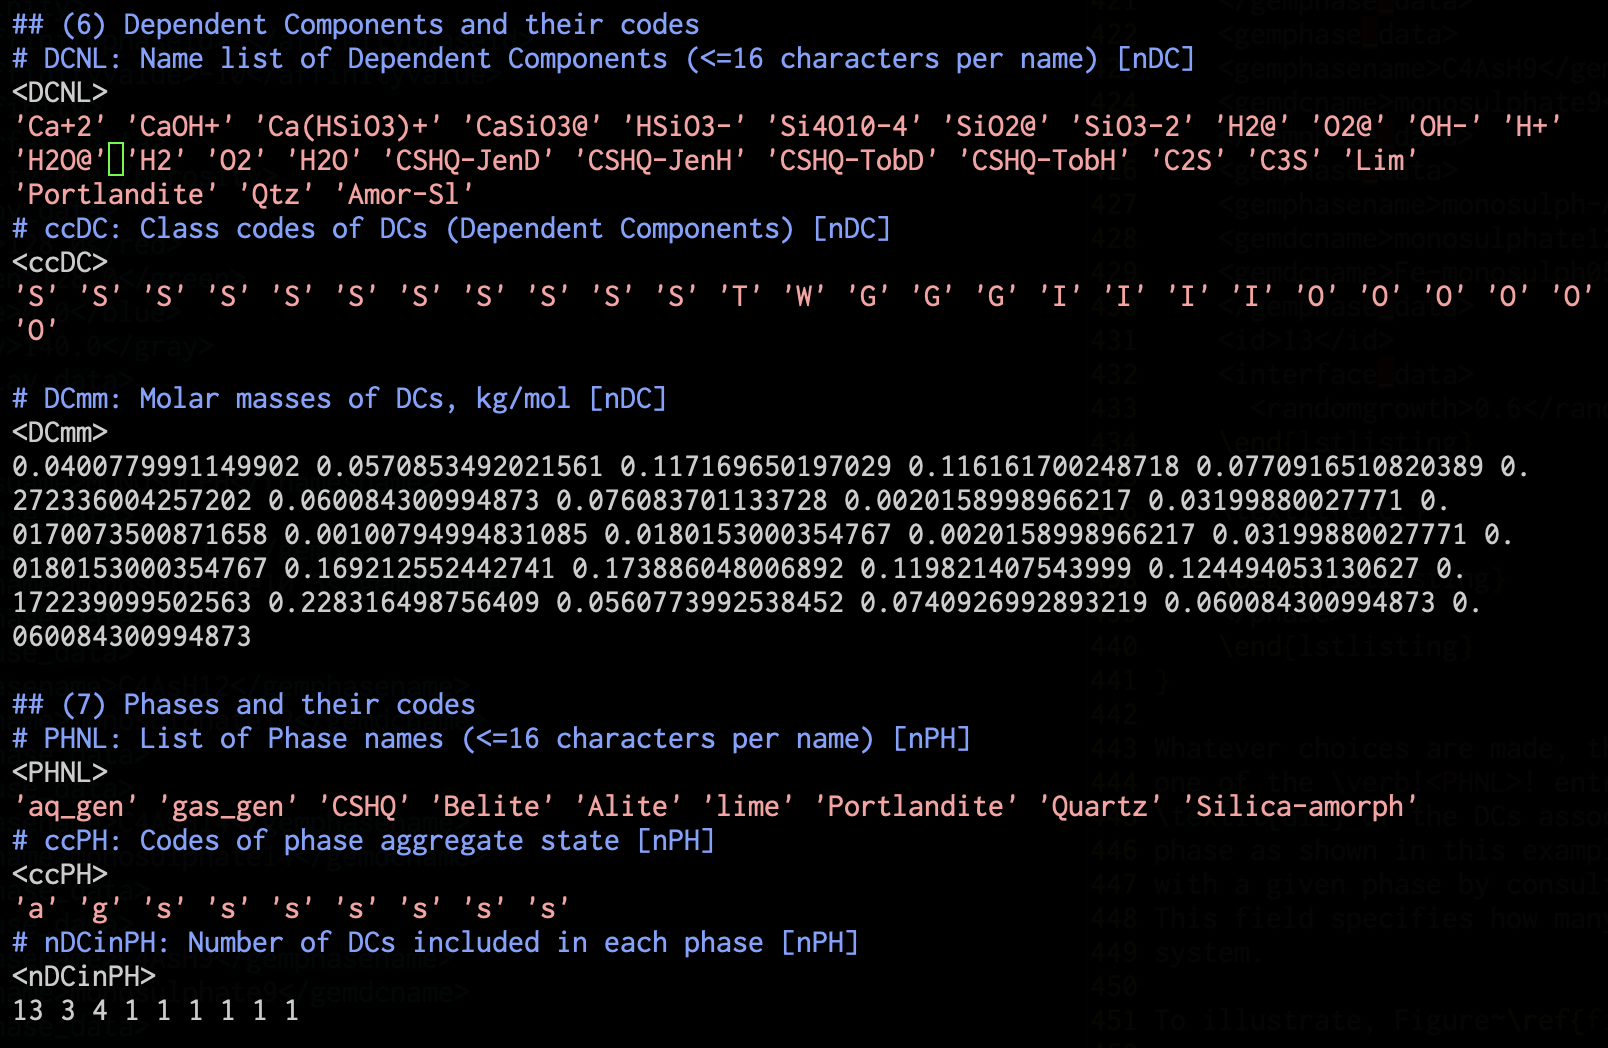
\includegraphics[width=0.7\textwidth]{Figures/dchfile.png}
	\caption{\label{fig:dchfile} Portion of a DCH input file showing the definitions
		of GEM phases and DCs.}
\end{figure}

\paragraph{Solid microstructure phases.} Solid microstructure
phases may be ``simple'' (one phase, one DC, and possibly
some impurities), ``solid solution'' (one phase, multiple DCs
that may be present in any mole fraction to give a phase
with nonstoichiometric composition, such as \ch{C-S-H} gel),
or ``composite'' (multiple thermodynamic phases combined for
simplicity or computational efficiency).

An example of a ``simple'' microstructure phase is alite,
which is usually a monoclinic form of tricalcium silicate
(\ch{Ca3SiO5}) with some impurities to stabilize the monoclinic
polymorph.
\scriptsize{
	\begin{lstlisting}
  {
    "thamesname": "Alite",
    "id": 2,
    "cement_component": 1,
    "interface_data": { }
    "gemphase_data": [
      {
        "gemphasename": "Alite",
        "gemdc": [{ "gemdcname": "C3S" }]
      }
    ],
    "impurity_data": {
      "k2ocoeff": 0.00087,
      "na2ocoeff": 0.0,
      "mgocoeff": 0.00861,
      "so3coeff": 0.007942
    },
    "kinetic_data": {
      .
      .
      .
    }
  },
 \end{lstlisting}
}

\normalsize{ }
This entry indicates three more features of a solid phase, namely
data about its interface with other phases, its impurity content,
and its kinetic behavior:
\begin{itemize}
	\item \verb!interface_data! in the above entry for alite
	      is empty, but can have information about the affinity the
	      phase has for growing on one or more other substrate phases, using
	      the name of the substrate phase and the thermodynamic contact
	      angle between the two:
	      \begin{itemize}
		      \item \verb!affinityphase! must be the \verb!thamesname! of
		            another \textit{microstructure} phase defined in this file
		      \item \verb!contactangle! is the equivalent thermodynamic
		            contact angle for the two phases in units of degrees,
		            and must be a real number on the interval $\left[0,180\right]$,
		            where \qty{0}{\degree} is perfect wetting and
		            \qty{180}{\degree} is complete nonwetting.
	      \end{itemize}
	\item \verb!impurity_data! contains data on the amounts
	      of four different possible impurities, namely
	      potassium, sodium, magnesium, and sulfur, in terms
	      of the \textit{mole fractions} of their equivalent oxides,
	      namely \ch{K2O}, \ch{Na2O}, \ch{MgO}, and \ch{SO3}.
	      Currently these are the only four impurities that
	      are recognized by THAMES.
	\item \verb!kinetic_data! is optional and will be described
	      in detail in a later section. For now, the presence of this
	      section indicates that the rates of reaction of this phase
	      will be controlled by a kinetic rate equation. If this
	      section is not provided, the amounts of this phase at any
	      time will be determined solely by thermodynamic equilibrium
	      as calculated by GEMS.
\end{itemize}

An example of a more complicated composite microstructure phase could
be a collection of carbonated AFm phases, which would include all the
monocarbonates, hemicarbonates, and tricarboaluminate phases:
\scriptsize{
	\begin{lstlisting}
      {
        "thamesname": "AFmc",
        "id": 14,
        "cement_component": 0,
        "interface_data": {
          "affinity": [
            { "affinityphase": "Alite", "contactanglevalue": 180 },
          ]
        },
        "gemphase_data": [
          {
            "gemphasename": "C4Ac0.5H105",
            "gemdc": [{ "gemdcname": "hemicarb10.5" }]
          },
          {
            "gemphasename": "C4Ac0.5H12",
            "gemdc": [{ "gemdcname": "hemicarb" }]
          },
          {
            "gemphasename": "C4Ac0.5H9",
            "gemdc": [{ "gemdcname": "hemicarb9" }]
          },
          {
            "gemphasename": "C4AcH11",
            "gemdc": [{ "gemdcname": "monocarb" }]
          },
          {
            "gemphasename": "C4AcH9",
            "gemdc": [{ "gemdcname": "monocarb9" }]
          }
        ]
      },
 \end{lstlisting}
}

\normalsize{ }
The absence of impurities or kinetic data in this example indicate
that the phase is to be considered pure and that its amount in the
microstructure at any time will be determined solely by thermodynamic
equilibrium with the electrolyte. Also note that each of the DCs
associated with this phase default to having zero porosity, so there
will be no subvoxel or interhydrate porosity associated with this
microstructure phase.

Finally, a solid solution with internal porosity can be defined, such
as \ch{C-S-H} gel:
\scriptsize{
	\begin{lstlisting}
      {
        "thamesname": "CSHQ",
        "id": 11,
        "cement_component": 0,
        "interface_data": {
          "affinity": [
            { "affinityphase": "Alite", "contactanglevalue": 30 },
            { "affinityphase": "AFmc", "contactanglevalue": 90 },
          ]
        },
        "gemphase_data": [
          {
            "gemphasename": "CSHQ",
            "gemdc": [
              { "gemdcname": "CSHQ-JenD", "gemdcporosity": 0.4935 },
              { "gemdcname": "CSHQ-JenH", "gemdcporosity": 0.4935 },
              { "gemdcname": "CSHQ-TobD", "gemdcporosity": 0.2004 },
              { "gemdcname": "CSHQ-TobH", "gemdcporosity": 0.2004 },
              { "gemdcname": "KSiOH", "gemdcporosity": 0.1825 },
              { "gemdcname": "NaSiOH", "gemdcporosity": 0.1825 }
            ]
          }
        ],
        "poresize_distribution": [
          { "diameter": 0.23228, "volumefraction": 0.01684781722375019 },
          { "diameter": 0.49089, "volumefraction": 0.02276126023357459 },
          .
          .
          .
        ],
        "Rd": [
          { "Rdelement": "K", "Rdvalue": 0.42 },
          { "Rdelement": "Na", "Rdvalue": 0.42 }
        ]
      },
\end{lstlisting}
}

\normalsize{ }
Two more sections can be found in this example. First, the pore size
distribution can be defined as a normalized probability density function,
with the differential volume fraction (\verb!volumefraction!, dimensionless)
given for each effective pore size dimension (\verb!diameter!) given in
nanometer units. The second new section is the impurity partition section,
with the name \verb!Rd!, that describes the proportion of impurities that will
be drawn from the surrounding electrolyte if available:
\begin{itemize}
	\item \verb!Rdelement! is the name of an independent component (IC)
	      found in the \verb!ICNL! section of the \verb!-dch.dat! file.
	\item \verb!Rdvalue! is the partition coefficient defined for
	      alkalis by Hong and Glasser (\textit{Cem Concr Res}, 29 (1999), 1893--1903;
	      \textit{Cem Concr Res}, 32 (2002), 1101-1111.) which is defined
	      \begin{equation}
		      R_\text{d} = \frac{c_s w}{c_d s} \qquad (\text{units of}\
		      \unit{\liter\per\kilo\gram})
	      \end{equation}
	      where $c_s$ is the concentration of the impurity in the solid phase
	      (units \unit{\mole\per\liter}), $c_d$ is the concentration of the impurity
	      in the electrolyte (units \unit{\mole\per\liter}), and $w/s$ is the
	      water-solids ratio in units of \unit{\liter\per\kilo\gram}
\end{itemize}

\subsubsection{\label{sec:timeparams} Calculation and output times}
The final section of this file is called \verb!time_parameters! and defines
both the final age of the material to simulate and the simulation times at
which THAMES should write data for visualization and for assessing the
pore size distribution and saturation state. This section is fairly simple:

\scriptsize{
	\begin{lstlisting}
  "time_parameters": {
    "finaltime": 56.0,
    "outtimes": [0.01, 0.1,0.5,1.0,3.0,7.0,14.0,28.0]
  }
\end{lstlisting}
}

\normalsize{ }
The meaning of the parameters are as follows:
\begin{itemize}
	\item \verb!finaltime! is the final time, in days, to attempt simulating
	      the microstructure evolution. For various reasons the simulation may not
	      complete the full requested age---for example, the microstructure could
	      be completely depleted of electrolyte and so not be able to perform any
	      other reactions---but the simulation will definitely stop
	      after this time is reached.
	\item \verb!outtimes! is a list of times, in days, at which THAMES should
	      output the microstructure state, which includes
	      \begin{itemize}
		      \item the full 3D microstructure image (an \verb!.img! file),
		      \item a 2D image of a slice of the microstructure (both \verb!.ppm!
		            and \verb!.png! files), and
		      \item the current pore size distribution and saturation state.
	      \end{itemize}
\end{itemize}

\end{document}
